\documentclass[aspectratio=169]{beamer}

% -------------------- Theme --------------------
\usetheme{Madrid}
\usecolortheme{default}
\setbeamertemplate{navigation symbols}{}
\setbeamertemplate{footline}[frame number]

% -------------------- Packages --------------------
\usepackage{amsmath,amssymb,bm}
\usepackage{booktabs}
\usepackage{graphicx}
\graphicspath{{../figures/blearner/}}
\usepackage{tikz}
\usetikzlibrary{arrows.meta,positioning,calc}

% -------------------- TikZ styles --------------------
\tikzset{
  treat/.style={circle, draw, thick, fill=blue!15, minimum size=8mm, align=center},
  outc/.style={circle, draw, thick, fill=orange!20, minimum size=8mm, align=center},
  conf/.style={circle, draw, thick, fill=purple!12, minimum size=8mm, align=center},
  hidden/.style={circle, draw, dashed, thick, fill=gray!10, minimum size=8mm, align=center},
  arrow/.style={-Latex, thick},
  note/.style={rectangle, rounded corners, draw, fill=yellow!12, align=center, font=\small}
}

% -------------------- Macros --------------------
\newcommand{\E}{\mathbb{E}}
\newcommand{\indep}{\perp\!\!\!\perp}
\newcommand{\ATE}{\mathrm{ATE}}
\newcommand{\CVaR}{\mathrm{CVaR}}

% -------------------- Metadata --------------------
\title[B-Learner]{B-Learner: Quasi-Oracle Bounds on Heterogeneous Causal Effects Under Hidden Confounding}
\subtitle{Causal Inference in the AI Era}
\author{Dan Vilenchik}
\institute{Ben-Gurion University of the Negev}
\date{\today}

\begin{document}

\begin{frame}
  \titlepage
\end{frame}

% ===================================================================
% PART 1
% ===================================================================

\begin{frame}{Today: two acts}
\begin{columns}
\column{0.52\textwidth}
\textbf{Part 1 — The paper}
\begin{itemize}\small
  \item Partial identification and bounds
  \item Sensitivity analysis lineage: ATE $\to$ CATE
  \item Tan's MSM ($\Lambda$); $\Lambda=2$ example
  \item Valid vs.\ sharp bounds; sharp CATE bounds
  \item Why CVaR = worst-case confounding
  \item Plug-in bias, pseudo-outcome, Neyman orthogonality
  \item Theorem 1: full bias bound
  \item Pointwise vs.\ average validity
  \item Empirical results
\end{itemize}

\column{0.46\textwidth}
\textbf{Part 2 — Referee mode}
\begin{itemize}\small
  \item Assumptions: tested vs.\ untested
  \item Limitations
  \item Comparison to classical methods
  \item Discussion
\end{itemize}
\end{columns}

\vspace{0.4em}
\begin{block}{Paper}
\small Oprescu et al.\ \emph{B-Learner: Quasi-Oracle Bounds on Heterogeneous Causal Effects Under Hidden Confounding.} ICML 2023.
\end{block}
\end{frame}

% ----- PROBLEM -----

\begin{frame}{The problem: CATE under hidden confounding}

\begin{columns}
\column{0.55\textwidth}
Standard CATE meta-learners (T-, X-, DR-Learner) require:
\[
  (Y(1),Y(0)) \indep T \mid X \quad\text{(unconfoundedness)}
\]
In practice there may be a hidden $U$ affecting both $T$ and $Y$. Unconfoundedness fails; any CATE estimate may be arbitrarily biased.

\medskip
\textbf{What can we do?}\\
Instead of a point estimate $\hat\tau(x)$, learn a bound:
\[
  [\,\hat\tau^-(x),\; \hat\tau^+(x)\,]
\]
that is \emph{provably valid} under a specified limit on how much $U$ can confound.

\column{0.42\textwidth}
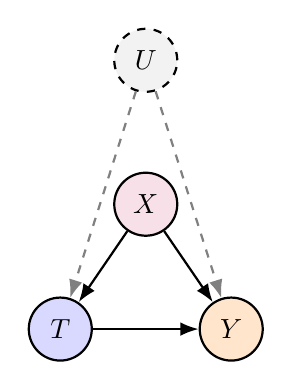
\begin{tikzpicture}[node distance=1.5cm]
  \node[conf] (X) {$X$};
  \node[treat, below left=1cm and 0.5cm of X] (T) {$T$};
  \node[outc, below right=1cm and 0.5cm of X] (Y) {$Y$};
  \node[hidden, above=1cm of X] (U) {$U$};
  \draw[arrow] (X) -- (T);
  \draw[arrow] (X) -- (Y);
  \draw[arrow] (T) -- (Y);
  \draw[arrow, gray, dashed] (U) -- (T);
  \draw[arrow, gray, dashed] (U) -- (Y);
\end{tikzpicture}

\vspace{0.4em}
\small Hidden $U$: unconfoundedness fails.\\
CATE estimate $\hat\tau(x)$ has unknown bias.
\end{columns}
\end{frame}

% ----- PARTIAL IDENTIFICATION -----

\begin{frame}{Key concept: partial identification and the identified set}

\begin{columns}
\column{0.54\textwidth}
\begin{block}{Point identification}
We can recover $\tau(x)$ exactly from observational data under unconfoundedness. The estimand is \textbf{a single value}.
\end{block}

\vspace{0.4em}
\begin{alertblock}{Partial identification}
When unconfoundedness fails, $\tau(x)$ is \textbf{not unique}.\\
Many DGPs are consistent with the data.\\
Each implies a different $\tau(x)$.\\[4pt]
The \textbf{identified set} is the set of all $\tau(x)$ values that some consistent DGP can produce.\\
A \textbf{bound} $[\tau^-(x), \tau^+(x)]$ characterizes this set.
\end{alertblock}

\column{0.44\textwidth}
\textbf{What do we need?}
\begin{itemize}
  \item An assumption that \emph{limits} (not eliminates) the hidden confounding
  \item Under that limit, the identified set becomes a bounded interval
\end{itemize}

\vspace{0.4em}
\begin{block}{Nuisance functions}
Intermediate functions we estimate not for their own sake, but because we need them to estimate $\tau(x)$:
\begin{itemize}\small
  \item Propensity score $e(x)$
  \item Outcome regression $\mu(x,a)$
  \item Quantile function $q(x,a)$ (new here)
\end{itemize}
\end{block}
\end{columns}
\end{frame}

% ----- LINEAGE -----

\begin{frame}{Where does B-Learner come from? Methodological lineage}

\begin{block}{Building block 1: Dorn, Guo \& Kallus (2021) --- sharp ATE bounds}
\small Derived \textbf{sharp} bounds on the average treatment effect under Tan's MSM.\\
Key tool: CVaR as the worst-case potential outcome distribution.\\
Provides the formula for $Y^+(x,a)$ that B-Learner builds on (our Result 1).
\end{block}

\smallskip
\begin{block}{Building block 2: Kallus \& Oprescu (2023) --- doubly-robust meta-learning}
\small Framework for doubly-robust, model-agnostic learning of \textbf{conditional} distributional effects.\\
Provides the Neyman-orthogonal pseudo-outcome construction and the second-stage regression machinery.
\end{block}

\smallskip
\begin{alertblock}{B-Learner (this paper)}
Combines both: applies Kallus \& Oprescu's efficient pseudo-outcome machinery to the Dorn et al.\ sharp ATE bound formula, \textbf{lifting ATE bounds to CATE bounds} with quasi-oracle rates, double robustness, and flexible learners.
\end{alertblock}
\end{frame}

% ----- MSM -----

\begin{frame}{Tan's Marginal Sensitivity Model (MSM)}

\begin{columns}
\column{0.57\textwidth}
Let $e(x) = P(T=1\mid X=x)$ be the \textbf{observed} propensity score.\\
Let $e(x,u) = P(T=1\mid X=x, U=u)$ be the \textbf{full} propensity (unobservable).

\medskip
\textbf{Assumption 1 (MSM):} There exists $\Lambda \geq 1$ such that:
\[
  \Lambda^{-1} \;\leq\; \frac{e(x,u)}{1-e(x,u)} \bigg/ \frac{e(x)}{1-e(x)} \;\leq\; \Lambda
\]

\medskip
The full odds of treatment can deviate from the observed odds by at most factor $\Lambda$.

\column{0.41\textwidth}
\begin{block}{Special cases}
$\Lambda = 1$:\; $e(x,u) = e(x)$ for all $u$\\
$\Rightarrow$ unconfoundedness holds.\\[4pt]
$\Lambda > 1$:\; hidden confounding allowed.\\
Larger $\Lambda$ = more confounding.
\end{block}

\vspace{0.3em}
\begin{block}{Relationship to Rosenbaum $\Gamma$}
\small $\Gamma$ bounds conditional odds between matched units. $\Lambda$ bounds marginal odds relative to observed propensity. Both are odds-ratio models; $\Lambda$ is more tractable for general regression-based estimation.
\end{block}
\end{columns}
\end{frame}

% ----- LAMBDA EXAMPLE -----

\begin{frame}{What does $\Lambda = 2$ mean? A concrete example}

\begin{columns}
\column{0.52\textwidth}
Suppose $e(x) = 0.5$ (observed odds $= 1$).\\[4pt]
Under $\Lambda = 2$: full odds $\in [1/2,\, 2]$, so
\[
  e(x,u) \;\in\; [1/3,\; 2/3]
\]
\textbf{Interpretation:} the hidden $U$ can shift treatment probability from 33\% to 67\% for someone with observed $e(x)=0.5$.

\medskip
Under $\Lambda = 4$: $e(x,u) \in [0.2,\; 0.8]$ — very wide uncertainty.

\medskip
\textbf{Rule of thumb:}\\
$\log\Lambda = 0.5 \Rightarrow \Lambda \approx 1.65$ (mild confounding)\\
$\log\Lambda = 1.0 \Rightarrow \Lambda \approx 2.72$ (moderate)\\
$\log\Lambda = 1.5 \Rightarrow \Lambda \approx 4.5$ (strong)

\column{0.46\textwidth}
\begin{block}{How to choose $\Lambda$?}
Two uses:
\begin{enumerate}
  \item \textbf{Domain knowledge}: ``How strong could the unmeasured confounder be?'' E.g.\ for 401(k), could unobserved savings habit triple treatment odds?
  \item \textbf{Breakdown analysis}: compute the $\Lambda$ at which the policy conclusion (e.g.\ CATE $> 0$) first fails. Ask: is this $\Lambda$ plausible?
\end{enumerate}
\end{block}

\vspace{0.2em}
\small Do \textbf{not} choose $\Lambda$ after seeing the results to confirm a desired conclusion --- that invalidates the analysis.
\end{columns}
\end{frame}

% ----- VALID VS SHARP -----

\begin{frame}{Valid vs.\ sharp bounds (Fig.~1)}

\begin{columns}
\column{0.52\textwidth}
\includegraphics[width=\textwidth]{fig1_bounds}

\smallskip\small
\textbf{Left:} true $\tau(x)$ (black) stays inside sharp bounds at $\log\Lambda=1.0$; outside at smaller $\Lambda$.\\
\textbf{Right:} sharp bounds (dashed) vs.\ valid bounds (dotted); blue = entire identified set.

\column{0.46\textwidth}
\begin{block}{Valid bound $\hat\tau^+(x)$}
Covers $\tau(x)$ for all DGPs consistent with data and MSM. May include impossible values --- overly cautious.
\end{block}

\vspace{0.4em}
\begin{alertblock}{Sharp bound $\tau^+(x)$}
The \emph{tightest} valid bound.\\
\textbf{Every} value inside is achievable by some consistent DGP.\\
Sharp bounds describe the identified set exactly --- no wasted space.
\end{alertblock}

\vspace{0.3em}
\small As $\Lambda \uparrow$: bounds widen.\\
At $\Lambda = 1$: bounds collapse to a point estimate (full identification).
\end{columns}
\end{frame}

% ----- RESULT 1 -----

\begin{frame}{The sharp CATE bounds (Result 1, from Dorn et al.\ 2021)}

Set $\alpha = \Lambda/(\Lambda+1) \in [0.5,1)$. The sharp CATE upper bound is $\tau^+(x) = Y^+(x,1) - Y^-(x,0)$:
\[
  Y^+(x,1) = e^*(x)\,\mu^*(x,1) + (1-e^*(x))\,\rho^+_*(x,1)
\]
\[
  Y^-(x,0) = (1-e^*(x))\,\mu^*(x,0) + e^*(x)\,\rho^-_*(x,0)
\]

\smallskip
\begin{columns}
\column{0.50\textwidth}
\textbf{Identifiable nuisances:}
\begin{itemize}\small
  \item $e^*(x)$: propensity score
  \item $\mu^*(x,a) = \E[Y\mid X{=}x, T{=}a]$: outcome regression
  \item $\rho^\pm_*(x,a)$: \textbf{CVaR} terms (see next slide)
\end{itemize}
\column{0.48\textwidth}
\begin{block}{Lower bound}
Swap $+\leftrightarrow -$ and $1\leftrightarrow 0$:
\[
  \tau^-(x) = Y^-(x,1) - Y^+(x,0)
\]
Full interval: $[\tau^-(x),\, \tau^+(x)]$.\\[4pt]
\small At $\Lambda=1$: $\rho^\pm_* = \mu^*$, so $\tau^+(x)=\tau^-(x)=\tau(x)$.
\end{block}
\end{columns}
\end{frame}

% ----- WHY CVaR -----

\begin{frame}{Why CVaR? Hidden confounding as a distributional tilt}

\textbf{Question:} what is the worst-case $\E[Y(1)\mid X=x]$ that the MSM allows?

\medskip
\begin{columns}
\column{0.54\textwidth}
\textbf{Treated group} ($T=1$, fraction $e(x)$):\\
We \emph{observe} their $Y(1)$.\\
The observed distribution $P(Y\mid X=x, T=1)$ is \textbf{fixed by the data} for any $Q \in \mathcal{M}(\Lambda)$.

\smallskip
\textbf{Untreated group} ($T=0$, fraction $1-e(x)$):\\
$Y(1)$ is \textbf{never observed}.\\
$U$ could have selected the units with \emph{highest} $Y(1)$ into the control group.\\
Under MSM, $U$ can tilt the selection by at most factor $\Lambda$ --- the worst case shifts mass to the \textbf{upper tail} of $Y(1)$.

\column{0.44\textwidth}
\begin{alertblock}{The worst-case reweighting}
The most extreme selection that $\Lambda$ allows places maximum probability on the upper $(1-\alpha)$ fraction of $Y$.\\[4pt]
This is exactly:
\[
  \CVaR_+(x,a) = \E[Y \mid Y \geq q^*_\alpha,\, X{=}x,\, T{=}a]
\]
the \textbf{expected value above the $\alpha$-quantile} (Conditional Value at Risk).
\end{alertblock}
\end{columns}
\end{frame}

% ----- CVaR DEFINITION -----

\begin{frame}{CVaR: formal definition and properties}

\begin{columns}
\column{0.54\textwidth}
\textbf{Definition.} $\CVaR_+(x,a)$ at level $\alpha = \Lambda/(\Lambda+1)$:
\[
  \CVaR_+(x,a) := \E\!\left[H_+\!\left(Z, q^*_+\right) \mid X=x, T=a\right]
\]
where the \emph{CVaR pseudo-outcome} is:
\[
  H_+(z, \bar q) = \bar q(x,a) + \frac{\{y - \bar q(x,a)\}_+}{1-\alpha}
\]
and $q^*_+(x,a)$ is the true $\alpha$-quantile of $Y\mid X=x, T=a$.

\medskip
The $\rho^+_*$ in Result 1 combines both:
\[
  \rho^+_*(x,a) = \Lambda^{-1}\mu^*(x,a) + (1-\Lambda^{-1})\,\CVaR_+(x,a)
\]

\column{0.44\textwidth}
\begin{block}{Financial analogy}
CVaR = ``Expected Shortfall'': average loss in the worst $\alpha$ fraction.\\[4pt]
Here: average $Y(1)$ in the tail that hidden $U$ could force into the control group.
\end{block}

\vspace{0.4em}
\begin{alertblock}{Effect of $\Lambda$}
$\Lambda\uparrow$ $\Rightarrow$ $\alpha\uparrow$ $\Rightarrow$ CVaR at more extreme quantile $\Rightarrow$ wider bounds.\\[4pt]
$\Lambda=1$: $(1-\Lambda^{-1})=0$, so $\rho^*_\pm = \mu^*$ (CVaR \emph{coefficient} is zero; the formula reduces without CVaR collapsing).
\end{alertblock}
\end{columns}
\end{frame}

% ----- DECOMPOSITION -----

\begin{frame}{Sharp bound = outcome regression + CVaR correction}

\[
  Y^+(x,1) =
  \underbrace{e(x)\,\mu(x,1)}_{\substack{\text{treated group: their $Y$ is observed}\\\text{fixed by data; no uncertainty here}}}
  \;+\;
  \underbrace{(1-e(x))\,\rho^+(x,1)}_{\substack{\text{untreated group: $Y(1)$ is counterfactual}\\\text{worst case = CVaR tail}}}
\]

\medskip
\textbf{Reading the formula:}
\begin{itemize}
  \item \textbf{Treated group} ($e(x)$ fraction): their $Y(1)$ is observed and matches $\mu(x,1)$. The observed distribution is pinned by data, leaving no room for adversarial tilt.
  \item \textbf{Untreated group} ($1-e(x)$ fraction): $Y(1)$ is missing. The MSM allows $U$ to have preferentially placed the highest-$Y(1)$ individuals into the untreated group. Worst case = $\rho^+(x,1)$ (CVaR blend).
\end{itemize}

\medskip
\begin{columns}
\column{0.48\textwidth}
\begin{block}{At $\Lambda=1$ (unconfounded)}
$\rho^+(x,1)=\mu(x,1)$, so $Y^+(x,1)=\mu(x,1)$.\\
Bounds collapse: full point identification.
\end{block}
\column{0.48\textwidth}
\begin{alertblock}{At large $\Lambda$}
CVaR moves toward the supremum of $Y$.\\
Bounds widen: conclusion becomes uncertain.
\end{alertblock}
\end{columns}
\end{frame}

% ----- PLUG-IN BIAS -----

\begin{frame}{Plug-in bias: why not just substitute estimated nuisances?}

A natural approach: estimate $\hat e$, $\hat\mu$, $\hat\rho$, then plug into Result 1:
\[
  \hat Y^+(x,1)_\text{plug-in} = \hat e(x)\,\hat\mu(x,1) + (1-\hat e(x))\,\hat\rho_+(x,1)
\]

\smallskip
\textbf{The problem.} Suppose $\|\hat e - e^*\| = n^{-1/4}$ and $\|\hat\rho_+ - \rho^+_*\| = n^{-1/4}$ (slow but typical rates in semiparametric models). The plug-in bias is first-order:
\[
  \hat Y^+(x,1)_\text{plug-in} - Y^+(x,1) \sim |\hat e - e^*| + |\hat\rho_+ - \rho^+_*| = O(n^{-1/4}) \to 0 \text{ slowly}
\]

\smallskip
\begin{alertblock}{Plug-in is biased for all $n$}
The bias does not vanish at $\sqrt{n}$ rate. The estimator is \textbf{inconsistent} at $\sqrt{n}$ and cannot achieve confidence intervals without shrinking bias away.
\end{alertblock}

\smallskip
\begin{block}{The fix: Neyman-orthogonal (doubly-robust) pseudo-outcomes}
Construct a corrected estimator whose bias is a \textbf{product} of nuisance errors: $|\hat e - e^*|\cdot|\hat\rho_+ - \rho^+_*|$. At $n^{-1/4}$ rates each, the product is $n^{-1/2}$ --- fast enough for $\sqrt{n}$-consistent estimation.
\end{block}
\end{frame}

% ----- NEYMAN ORTHOGONALITY -----

\begin{frame}{Neyman orthogonality and cross-fitting}

\begin{columns}
\column{0.53\textwidth}
\textbf{Neyman-orthogonal score:}\\
An estimating equation $m(\tau, \eta)$ is Neyman-orthogonal if:
\[
  \partial_\eta m(\tau^*, \eta^*)\bigl[\hat\eta - \eta^*\bigr] = 0
\]
The score is \emph{first-order insensitive} to nuisance estimation errors.

\medskip
\textbf{Effect:} the remaining bias is second-order (a product of rates), not first-order.

\medskip
\textbf{Cross-fitting} (K-fold):
\begin{enumerate}\small
  \item Split data into $K$ folds.
  \item Estimate nuisances on fold $-k$ (held-out).
  \item Compute pseudo-outcomes on fold $k$ only.
\end{enumerate}
Decouples nuisance training from pseudo-outcome evaluation $\Rightarrow$ avoids overfitting.

\column{0.45\textwidth}
\begin{block}{Quasi-oracle rate}
When nuisances converge at $n^{-1/4}$:\\[4pt]
Bias $\lesssim$ product $= n^{-1/4} \cdot n^{-1/4} = n^{-1/2}$\\[4pt]
So the second-stage estimator converges at the rate it would if the nuisances were \emph{exactly known} (oracle).\\[4pt]
This is the \textbf{quasi-oracle property}.
\end{block}

\vspace{0.4em}
\begin{alertblock}{Why $n^{-1/4}$?}
\small Typical nonparametric rate in moderate dimensions. Both $\hat e$ and $\hat\rho_+$ must achieve this for the product-of-rates guarantee.
\end{alertblock}
\end{columns}
\end{frame}

% ----- PSEUDO-OUTCOME -----

\begin{frame}{The B-Learner pseudo-outcome (Definition 2)}

\begin{columns}
\column{0.56\textwidth}
Applying the Kallus \& Oprescu (2023) machinery to the Dorn et al.\ bound formula gives:
\begin{align*}
  \phi^+_1(Z,\hat\eta) &= TY + (1-T)\hat\rho_+(X,1)\\
  &\quad+ \tfrac{(1-\hat e(X))\,T}{\hat e(X)}\bigl(R_+(Z,\hat q_+) - \hat\rho_+(X,1)\bigr)
\end{align*}
\vspace{-0.8em}
\[
  \phi^+_\tau(Z,\hat\eta) = \phi^+_1(Z,\hat\eta) - \phi^-_0(Z,\hat\eta)
\]

\smallskip
\begin{block}{What the IPW correction does}
\small The term $\tfrac{(1-\hat e)T}{\hat e}(\cdot)$ reweights treated units to represent the untreated group's counterfactual. This is the first-order correction that makes the score Neyman-orthogonal.
\end{block}

\column{0.42\textwidth}
\begin{block}{Double robustness: validity}
\small Bounds remain \textbf{valid} if either $\hat e \to e^*$ or $\hat\rho_+ \to \rho^+_*$ (one consistent nuisance suffices to cancel the product-of-rates bias).
\end{block}

\vspace{0.4em}
\begin{alertblock}{Sharpness requires more}
\small For \textbf{sharp} bounds, quantile estimates $\hat q_\pm$ must also be consistent. If $(\hat q_+ - q^+_*)^2 \not\to 0$, bounds remain valid but are no longer sharp --- they become conservative.
\end{alertblock}

\vspace{0.4em}
\small At $\Lambda=1$: reduces to the DR-Learner pseudo-outcome exactly.
\end{columns}
\end{frame}

% ----- ALGORITHM -----

\begin{frame}{B-Learner: the two-stage algorithm}

\begin{columns}
\column{0.55\textwidth}
\textbf{Stage 1: nuisance estimation} (K-fold cross-fitting)
\begin{enumerate}\small
  \item Estimate propensity $\hat e(x)$
  \item Estimate outcome regression $\hat\mu(x,a)$
  \item Estimate quantile $\hat q_\pm(x,a)$ at level $\alpha$
  \item Construct $\hat\rho_\pm(x,a) = \Lambda^{-1}\hat\mu + (1-\Lambda^{-1})\widehat{\CVaR}_\pm$
\end{enumerate}

\vspace{0.5em}
\textbf{Stage 2: bounds regression}
\begin{enumerate}\small
  \setcounter{enumi}{4}
  \item Compute pseudo-outcomes $\hat\phi^\pm_\tau(Z_i, \hat\eta^{(k)})$ on each fold
  \item Regress pseudo-outcomes on $X$ using any learner $\mathbb{E}_n$
  \item Output $\hat\tau^+(x)$ and $\hat\tau^-(x)$
\end{enumerate}

\column{0.43\textwidth}
\begin{block}{Flexibility}
Any learner for each stage: RF, NN, linear, kernel. Notation:
$\hat\tau^+(\{1^\text{st}\}, \{2^\text{nd}\})$, e.g.\ $\hat\tau^+(\text{RF},\text{RF})$.
\end{block}

\vspace{0.4em}
\begin{block}{Course connection}
Stage 2 is identical to the DR-Learner, but with bounds pseudo-outcomes $\hat\phi^\pm_\tau$ instead of CATE pseudo-outcomes.
\end{block}

\vspace{0.3em}
\small Extra cost vs.\ DR-Learner: quantile regression in Stage 1.
\end{columns}
\end{frame}

% ----- THEOREM 1 -----

\begin{frame}{Theorem 1: the full bias bound}

\begin{block}{Theorem 1 (Pseudo-outcome Conditional Neyman Orthogonality)}
Under Assumption 2 (boundedness), the absolute bias $|\mathcal{E}^+_\tau(x;\hat\eta)|$ of the CATE upper-bound pseudo-outcome satisfies:
\[
  |\mathcal{E}^+_\tau| \;\lesssim\;
  \underbrace{|\hat e - e^*|\cdot|\hat\rho_+(x,1) - \rho^+_*(x,1)|}_{\text{treatment side}}
  \;+\;
  \underbrace{(\hat q_+(x,1) - q^+_*(x,1))^2}_{\text{quantile, treatment}}
\]
\[
  \quad + \underbrace{|\hat e - e^*|\cdot|\hat\rho_-(x,0) - \rho^-_*(x,0)|}_{\text{control side}}
  \;+\;
  \underbrace{(\hat q_-(x,0) - q^-_*(x,0))^2}_{\text{quantile, control}}
\]
\end{block}

\smallskip
\begin{columns}
\column{0.50\textwidth}
\begin{alertblock}{Three terms, two mechanisms}
\small \textbf{Product terms}: vanish if either $\hat e$ or $\hat\rho$ is consistent on the respective side.\\
\textbf{Squared quantile terms}: independent of $\hat e$ --- must converge on their own.
\end{alertblock}
\column{0.48\textwidth}
\begin{block}{Implication}
\small \textbf{Validity}: one of $\hat e$ or $\hat\rho_+$ consistent $\Rightarrow$ product terms vanish.\\
\textbf{Sharpness}: also need $\hat q_\pm \to q^*_\pm$.\\
Applies independently to both sides.
\end{block}
\end{columns}
\end{frame}

% ----- POINTWISE VS AVERAGE -----

\begin{frame}{Pointwise vs.\ average validity: an important subtlety}

\begin{block}{What Corollary 1 (ERM, in the paper) actually gives}
For an ERM second-stage regression over a function class $\mathcal{F}$, validity holds \textbf{on average}:
\[
  \frac{1}{n}\sum_{i=1}^n \bigl[\hat\tau^+(X_i) - \tau^+(X_i)\bigr] \;\geq\; -o_p(1)
\]
The estimated bound covers the true bound \emph{in aggregate over the sample}, not necessarily at every individual $x$.
\end{block}

\smallskip
\begin{columns}
\column{0.50\textwidth}
\begin{alertblock}{Pointwise validity requires more}
\small For $\hat\tau^+(x) \geq \tau^+(x) - o_p(1)$ at every $x$: Appendix C.2 shows this holds for \textbf{linear smoothers} only. General ERM (e.g.\ random forests) does not guarantee it.
\end{alertblock}
\column{0.48\textwidth}
\begin{block}{What this means in practice}
\small CATE bounds are most useful \emph{per individual} --- this requires pointwise validity.\\[2pt]
\textbf{Use linear smoothers} in Stage 2 for pointwise guarantees. With ERM, interpret as average-valid only.
\end{block}
\end{columns}
\end{frame}

% ----- SYNTHETIC RESULTS A -----

\begin{frame}{Empirical results: quasi-oracle convergence (Fig.~2a)}
\vspace{-0.5em}
\begin{center}
  \includegraphics[width=0.68\textwidth]{fig2a_oracle}
\end{center}
\vspace{-0.3em}
\small
\textbf{B-Learner (RF,RF)} vs.\ oracle ($\hat\tau^+$ with true nuisances) vs.\ plug-in.\\[2pt]
\textbf{Key observation:} B-Learner and oracle converge at the \emph{same rate} (parallel lines, log-log scale). The plug-in is biased for every $n$.\\
This confirms the quasi-oracle property --- with a few hundred samples, B-Learner already performs nearly as well as if it knew the propensity and CVaR exactly.
\end{frame}

% ----- SYNTHETIC RESULTS B -----

\begin{frame}{Empirical results: comparison to competitors (Fig.~2b)}
\vspace{-0.5em}
\begin{center}
  \includegraphics[width=0.68\textwidth]{fig2b_competitors}
\end{center}
\vspace{-0.3em}
\small
\textbf{B-Learner} vs.\ \textit{Sensitivity Kernel} (Gaussian kernel nuisances) and \textit{Quince} (Bayesian NN).\\[2pt]
Using the same nuisances (GK), B-Learner is comparable to \textit{Sensitivity Kernel}.\\
With NN or RF nuisances, B-Learner outperforms GK-based competitors --- confirming that learner flexibility matters.
\end{frame}

% ----- IHDP -----

\begin{frame}{Empirical results: IHDP deferral policy (Fig.~3)}
\begin{columns}
\column{0.50\textwidth}
\begin{center}
  \includegraphics[width=\textwidth]{fig3_ihdp}
\end{center}
\column{0.48\textwidth}
\textbf{Setting:} IHDP with hidden confounding.\\
\textbf{Policy:} recommend treatment if $[\hat\tau^-, \hat\tau^+]$ excludes zero; defer to expert otherwise.\\[4pt]
\textbf{x-axis:} deferral rate (fraction deferred).\\
\textbf{y-axis:} recommendation error rate (log scale).

\smallskip
\begin{alertblock}{Result}
B-Learner (NN,NN) matches \textit{Quince}.\\
B-Learner (RF,RF) outperforms GK-based \textit{Sensitivity Kernel}.\\
Mixing NN Stage 1 with RF Stage 2 also works well --- a unique advantage of the meta-learner design.
\end{alertblock}
\end{columns}
\end{frame}

% ----- 401K -----

\begin{frame}{Real data: 401(k) eligibility and wealth (Fig.~4)}
\begin{columns}
\column{0.44\textwidth}
\begin{center}
  \includegraphics[width=\textwidth,height=0.38\textheight,keepaspectratio]{fig4_401k}
\end{center}
\vspace{-0.2em}
{\scriptsize
\begin{block}{How to read this figure}
\begin{itemize}
\setlength\itemsep{0pt}\setlength\parsep{0pt}
  \item \textbf{T:} 401(k) eligibility.\quad\textbf{Y:} net financial assets.
  \item \textbf{Confounder:} unobserved saving preference.
  \item Left panel at $\log\Lambda\!=\!0.2$: each person gets $[\tau^-(x),\tau^+(x)]$.
  \item $\tau^-(x)>0 \Rightarrow$ effect \textbf{robust} at this confounding level.
  \item $\tau^-(x)\leq 0 \Rightarrow$ data do not rule out zero/negative effect.
\end{itemize}
\end{block}}

\column{0.54\textwidth}
\begin{block}{Left ($\log\Lambda=0.2$)}
\small Distribution of lower/upper CATE bounds across individuals.\\
Most lower bounds positive $\Rightarrow$ likely real positive effect at low confounding.
\end{block}

\smallskip
\begin{block}{Right (varying $\Lambda$) --- breakdown analysis}
\small As $\Lambda$ grows, bounds widen; we track what fraction of lower bounds
cross zero, asking how strong unobserved saving preference must be before
the conclusion of a positive effect fails.\\[3pt]
At $\log\Lambda\approx 0.5$: ${\sim}50\%$ of lower bounds turn negative.\\
\textbf{Breakdown question:} is $\log\Lambda=0.5$ plausible here?
\end{block}
\end{columns}
\end{frame}

% ----- COMMON MISTAKE -----

\begin{frame}{Common mistake: ``Confidence intervals already handle this''}

\begin{alertblock}{What CI's do \emph{not} capture}
DR-Learner CIs quantify \textbf{statistical} uncertainty (finite-sample noise).\\
They assume unconfoundedness is true and \emph{shrink} with $n$.\\[4pt]
$\hat\tau(x) \pm 1.96\,\mathrm{se}$ narrows as $n\to\infty$ --- but converges to the \emph{wrong} $\tau(x)$ if $U$ exists.
\end{alertblock}

\smallskip
\begin{block}{What CATE bounds capture}
$[\hat\tau^-(x), \hat\tau^+(x)]$ quantifies uncertainty from \textbf{hidden confounding}.\\
This uncertainty does \emph{not} shrink with $n$ if $U$ is unresolvable (unidentifiability persists).\\
The two types of uncertainty are orthogonal --- both are needed for trustworthy causal claims.
\end{block}

\smallskip
\begin{alertblock}{Second trap: pointwise vs.\ average validity}
An ERM second stage gives average-valid bounds, not pointwise-valid ones. Do not interpret individual bounds as guaranteed to cover the true $\tau(x)$ pointwise without verifying the smoother conditions.
\end{alertblock}
\end{frame}

% ===================================================================
% PART 2: REFEREE MODE
% ===================================================================

\begin{frame}{}
\begin{center}
\vspace{1em}
{\Large \textbf{Part 2: Referee Mode}}

\vspace{1em}
{\large Reading the paper as a peer reviewer}
\end{center}
\end{frame}

% ----- ASSUMPTIONS -----

\begin{frame}{Assumptions: tested vs.\ untested}

\small
\begin{tabular}{p{3.8cm}p{2.2cm}p{4.2cm}}
\toprule
\textbf{Assumption} & \textbf{Status} & \textbf{Comment} \\
\midrule
MSM correctly models confounding & \textcolor{red}{Untested} & Observationally indistinguishable from alternatives \\
Positivity $e(x)\!\in\!(\epsilon,1{-}\epsilon)$ & Assumed & Standard; IPW unstable near boundaries \\
Consistency $Y=Y(T)$ & Assumed & SUTVA; not discussed \\
$\Lambda$ set correctly & \textcolor{red}{User choice} & No data-driven selection method \\
Nuisance boundedness & Assumed & Required for Neyman-orthogonality theory \\
Quantile accuracy & Partial & Needed for sharpness (not just validity) \\
\bottomrule
\end{tabular}
\normalsize

\smallskip
\begin{block}{The hardest assumption}
\small The MSM, Rosenbaum $\Gamma$, e-value, and partial $R^2$ models all give \emph{different} bounds under the same data. The choice of sensitivity model is itself untested and shapes all conclusions.
\end{block}
\end{frame}

% ----- LIMITATIONS -----

\begin{frame}{Limitations acknowledged and not acknowledged}

\textbf{Acknowledged:}
\begin{itemize}\small
  \item \textbf{Binary treatment only} ($T\in\{0,1\}$): continuous and multi-valued $T$ not covered.
  \item \textbf{$\Lambda$ is user-specified}: too small $\Rightarrow$ invalid; too large $\Rightarrow$ vacuous.
  \item \textbf{Rate requires $n^{-1/4}$ nuisances}: slow in high-dimensional $X$.
\end{itemize}

\smallskip
\textbf{Not addressed:}
\begin{itemize}\small
  \item \textbf{Pointwise validity}: ERM Stage 2 gives only average-valid bounds (see Appendix C.2 for linear-smoother case).
  \item \textbf{Simultaneous validity across all $x$}: no family-wise error control.
  \item \textbf{Sensitivity model selection}: no method for choosing between MSM and alternatives.
  \item \textbf{Computational cost}: quantile regression in Stage 1 is more expensive than mean regression.
  \item \textbf{Limited empirical improvement}: B-Learner only matches \textit{Quince} in practice despite stronger theory.
\end{itemize}
\end{frame}

% ----- COMPARISON -----

\begin{frame}{Comparison to related methods}

\small
\begin{tabular}{p{2.8cm}p{2.8cm}p{3.0cm}p{2.2cm}}
\toprule
\textbf{Method} & \textbf{Target} & \textbf{Properties} & \textbf{Flexibility} \\
\midrule
Rosenbaum sensitivity & ATE bound & Valid & Matched pairs \\
Sensitivity Kernel & CATE bound & Valid & GK only \\
Quince (Jesson 2021) & CATE bound & Valid & BNN only \\
\midrule
\textbf{B-Learner} & CATE bound & Valid + sharp + quasi-oracle + doubly robust & Any learner \\
\bottomrule
\end{tabular}
\normalsize

\smallskip
\textbf{Where B-Learner wins:} learner flexibility, theoretical guarantees (sharpness, quasi-oracle rate), both-sides bias bound.

\smallskip
\textbf{Practical caveat:} B-Learner(NN,NN) and \textit{Quince} perform similarly in Fig.~3. Theoretical superiority does not always translate to empirical gains on small datasets.
\end{frame}

% ----- DISCUSSION -----

\begin{frame}{Discussion questions}

\begin{enumerate}
  \item At $\log\Lambda=0.6$, about half of 401(k) CATE lower bounds turn negative. \textbf{Does this mean the 401(k) effect is confounded?} What additional evidence would distinguish confounding from sampling variability?

  \medskip
  \item The quasi-oracle property guarantees B-Learner converges at the oracle rate. \textbf{Does this mean B-Learner is safe to use on 200 observations?} What does the asymptotic constant hide?

  \medskip
  \item Suppose you use bounds $[\hat\tau^-(x), \hat\tau^+(x)]$ to decide who gets a treatment. \textbf{How would you operationalize the decision?} What role does $\Lambda$ play in the decision rule?

  \medskip
  \item ERM in Stage 2 gives average-valid bounds, not pointwise-valid ones. \textbf{When does this matter?} Can you give a decision-making scenario where average validity is sufficient?

  \medskip
  \item At $\Lambda=1$, B-Learner reduces to DR-Learner. \textbf{What does this tell us about unconfoundedness?} Is it the same as saying the identified set is a single point?
\end{enumerate}
\end{frame}

% ----- TAKE-AWAY -----

\begin{frame}{Take-away}

\textbf{Core contribution:}
\[
  \hat\tau^+(x),\; \hat\tau^-(x) \;\approx\; \tau^+(x),\; \tau^-(x)
\]
\textit{sharp CATE bounds under the MSM, at quasi-oracle rates, using any nuisance learner.}

\medskip
\begin{columns}
\column{0.48\textwidth}
\begin{block}{What it contributes}
\begin{itemize}\small
  \item First CATE sensitivity method: valid + sharp + efficient + doubly robust
  \item Lineage: Dorn et al.\ (ATE bounds) + Kallus \& Oprescu (DML machinery) $\to$ CATE bounds
  \item At $\Lambda=1$: reduces to DR-Learner
  \item Practical: bounds widen with $\Lambda$, narrow with $n$
\end{itemize}
\end{block}

\column{0.48\textwidth}
\begin{alertblock}{What remains open}
\begin{itemize}\small
  \item Continuous and multi-valued treatments
  \item Data-driven selection of $\Lambda$
  \item Pointwise validity guarantees for ERM Stage 2
  \item Sharpness under alternative sensitivity models
  \item Behavior under covariate shift
\end{itemize}
\end{alertblock}
\end{columns}
\end{frame}

\end{document}
